\documentclass[a4paper]{scrreprt}

%% Language and font encodings
\usepackage[french, english]{babel}
\usepackage[utf8x]{inputenc}
\usepackage[T1]{fontenc}

%% Sets page size and margins
\usepackage[a4paper,top=3cm,bottom=2cm,left=3cm,right=3cm,marginparwidth=1.75cm]{geometry}

%% Useful packages
\usepackage{amsmath}
\usepackage{graphicx}
\usepackage[colorinlistoftodos]{todonotes}
\usepackage[colorlinks=true, allcolors=blue]{hyperref}

\title{Cthulhu vs Satan\footnote{Nom provisoire}}
\subtitle{Tactical-RPG}
\date{Octobre 2018}
\author{Simon \textsc{Gigant}, Clément \textsc{Leb\oe uf}, Fabien \textsc{Matusalem}}
%\titlehead{\centering
\includegraphics[width=6cm]{test}}


\begin{document}
\maketitle
\null\vfill
\noindent
Game Design Document\\
Version v0.1, Oct 2018\\
\newpage

\begin{abstract}
Affrontez l'IA dans ce jeu de stratégie au tour par tour, créez une stratégie pour éliminer l'équipe adverse ou invoquer votre divinité le premier pour remporter la partie.
\end{abstract}

\tableofcontents

% ______________________
% chapter Overview
% ______________________
\chapter{Aperçu}

\section{Le Concept}
Le jeu s'inspire des échecs et des jeux de rôle tactiques, et implémentera une intelligence artificielle. Le but d'un joueur est de déplacer deux de ses personnages dans les deux zones de but du camp adverse.

% \section{Unique Selling Point}
% describe you unique selling point in one paragraph


% ______________________
% chapter References
% ______________________

\chapter{Références}
Le jeu s'inspire des échecs pour l'aspect des informations données au joueur ; Chaque joueur devra avoir une information complète du jeu adverse (positions des pions, type de pion, temps de recharge des compétences...). Le côté stratégique du positionnement des pions s'appuyera aussi sur le jeu d'échecs.
Le système de combat s'appuyera sur les faiblesses/resistances qu'on peut retrouver dans Pokémon ou Fire Emblem.
Le système de déplacement avec une action possible parmi plusieurs est inspiré de nombreux tactical RPG dont le Dofus ou Chroma Squad.

% ______________________
% chapter Specification and Market Analysis
% ______________________

\chapter{Spécifications}
Ce jeu est destiné à des joueurs patients qui veulent perfectionner leurs stratégies en affrontant une IA.

\section{Joueurs}

Le jeu se jouera à 1 (contre l'IA) ou 2 joueurs (l'un contre l'autre).

\section{Genre}
Le jeu est un jeu de rôle tactique (tactical RPG). C'est-à-dire un jeu en tour par tour où des pions se déplacent sur un quadrillage et peuvent attaquer leurs adversaires.

\section{Direction artistique}
Les graphismes seront faits en pixel art, avec une palette de couleurs réduite à part la couleur de l'équipe du personnage afin de maximiser la visibilité.
Les références visuelles sont The Shrouded Isle (pour l'ambiance générale et les couleurs), Chroma Squad (pour l'aspect isométrique et pixel art basse résolution), et Bloodborne (pour le character design des monstres).

Les musiques seront lourdes et angoissantes comme le travail de Richard Vreeland pour la bande son de It follows.

\begin{figure}
\centering
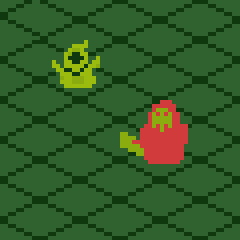
\includegraphics[width=0.3\textwidth]{example.png}
\caption{\label{fig:art} Exemple rapide d'art}
\end{figure}

\section{Formes d'engagement}

L'engagement principal du jeu sera le challenge proposé par le duel contre l'IA, mais d'abord la découverte des mécaniques de jeu et des stratégies à mettre en place pour vaincre l'IA.

% ______________________
% chapter Game Details
% ______________________


\chapter{Gameplay et cadre de jeu}

\section{Ambiance et émotions}

Le jeu doit inspirer de la réflexion et des réactions aux actions adverses, tout en donnant un cadre d'apocalypse et de chaos qui inspire la désolation.

\section{Histoire}

Deux cultes essayent d'effectuer leur rituel pour invoquer leur déité. Le premier des cultes à placer un cultiste dans chacune des zones nécessaires au rituel prendra le contrôle du monde.

\section{Monde/Environnement}

Le jeu se place sur Terre, dans un univers moderne, proche de l'\oe uvre de Howard Phillip Lovecraft.

\section{Personnages en jeu}
Les personnages seront exclusivement des cultistes ainsi que Cthulhu et Satan.

\section{Objectif principal}

L'unique objectif est de gagner la partie, il n'y a pas d'objectif global extrinsèque, intrinsèquement le joueur voudra améliorer ses stratégies.

\section{Mécaniques principales}

La mécanique principale de jeu est le déplacement et les actions entreprises par les personnages.

Il existe 3 types de personnages :
\begin{itemize}
    \item Les tanks : Ils peuvent encaisser plus de dégâts avant de mourir, et bloquer le déplacement d'adversaires proches.
    \item Les soutiens : Ils peuvent déplacer leurs alliés et leurs ennemis.
    \item Les attaquants : Ils se déplacent plus vites que les autres unités mais sont assez fragiles.
\end{itemize}

\section{Contrôles}
Le jeu se jouera exclusivement à la souris, avec le clic gauche pour interagir.

% ______________________
% chapter Front End
% ______________________


\chapter{Menus}

\section{\'Ecran d'accueil}

L'écran principal indiquera le nom du jeu, des crédits ainsi que les boutons "1 Joueur", "2 Joueurs", "Options" et "Quitter".

\section{Menus}

Le menu d'options pourra proposer de couper le son.
Lorsqu'on choisit "1 Joueur", on pourra choisir la difficulté de l'IA ou revenir au menu principal.

\section{\'Ecran de fin}

Une fois une partie terminée, un récapitulatif de la partie affichera le nombre de tours joués ainsi que le joueur qui a gagné.

% ______________________
% chapter Game Details
% ______________________


\chapter{Technologie}


\section{Plateformes visées}
Les plateformes visées sont Linux et Windows.

\section{Matériel}

Le jeu ne nécessite qu'une souris.

\section{Outils et systèmes de développement}
Le jeu est conçu avec le langage C++ et la bibliothèque "Gamedev Framework". 
Nous utiliserons un éditeur de texte pour le code, Aseprite pour les sprites et animations, FL Studio et Maschine pour la musique et le sound design et \LaTeX pour la mise en page des documents annexes (celui-ci, le rapport de projet ainsi que le support de soutenance).
La gestion du projet utilise des outils tels que Trello, Git, Github, Overleaf et Discord.

% ______________________
% chapter Game Details
% ______________________


\chapter{Sujets et inclusivité}

\section{Inclusivité}

Le jeu mettra en avant des personnages diversifiés en sexe, et aux origines et sexualités indéterminables.

\section{Accessibilité}
Le jeu ne demande pas de réflexe ni des contrôles complexes, il sera donc accessible aux joueurs avec des problèmes de motricité.
Ses visuels utiliseront des couleurs facilement distingables pour les 2 équipes, ainsi que des indices visuels non liés à la couleur, afin de faciliter l'accès au jeu pour les joueurs ayant des difficultés à reconnaître les couleurs.
Le son ne sera aucunement nécessaire, les joueurs avec une audition réduite pourront y jouer sans problème.

% ______________________
% chapter Game Details
% ______________________


\chapter{Planning}

\begin{table}[h]
\centering
\begin{tabular}{|l|l|l|}
\hline
Milestone & Description & Date \\\hline
& Date de départ & 9 octobre 2018 \\
1 & Conception et architecture  & 1 novembre 2018 \\
2 & Mécaniques de jeu & 15 janvier 2019\\
3 & Intelligence Artificielle & 1 février 2019. \\
& Fin du projet & mars 2019 \\
\hline
\end{tabular}
\caption{\label{tab:schedule}Planning prévisionnel.}
\end{table}


% ______________________
% chapter Game Details
% ______________________


\chapter{Crédits}

Ce jeu est conçu et développé par Simon Gigant, Clément Leb\oe uf et Fabien Matusalem.

%\todo[inline, color=green!40]{This is an inline comment.}

%\bibliographystyle{alpha}
%\bibliography{sample}

\end{document}
